\section{Introduction}

Speech technology has made much progress over the past decade~\citep{chan2015las,graves2006ctc,baevski2020wav,radford2022whisper} and has been integrated into many consumer products, such as home assistants and smartphones.
Despite this progress, speech technology is still absent for the vast majority of the over 7,000 languages spoken around the world~\citep{lewis2016ethnologue}.
Moreover, many of these languages are at risk of disappearing by the end of this century and the narrow language coverage of current technology may contribute to this trend~\citep{bromham2021disappear}.

Speech models have traditionally been built by training models on large amounts of labeled training data which is only available for a small number of languages.
More recently, self-supervised speech representations have dramatically lowered the amount of labeled data required to build speech systems~\citep{oord2018cpc,schneider2019wav2vec,baevski2020wav}.
But despite this progress, prominent recent work still only supports about 100 languages~\citep{radford2022whisper,zhang2023usm}.

To address this, we build a new dataset comprising a moderate amount of labeled data for \nummmslang{} languages and another dataset of unlabeled speech in \numgrnlang{} languages (\textsection\ref{sec:datasets}). 
We leverage this data to pre-train wav2vec 2.0 models supporting several times more languages than any known prior work (\textsection\ref{sec:pretrain}) and then fine-tune these models to build a multilingual speech recognition model supporting \nummmslang{} languages (\textsection\ref{sec:asr}), language identification models for \numlidlang{} languages (\textsection\ref{sec:lid}) and text-to-speech models for \nummmslang{} languages (\textsection\ref{sec:tts}). 

The Massively Multilingual Speech (MMS) project aims to expand speech technology to many more people and we hope that it can be a small contribution to preserving the languages diversity of this world.
\autoref{fig:map} illustrates the location where the languages supported in this work are spoken and which tasks we cover for each language.



\begin{figure}[t]
\centering
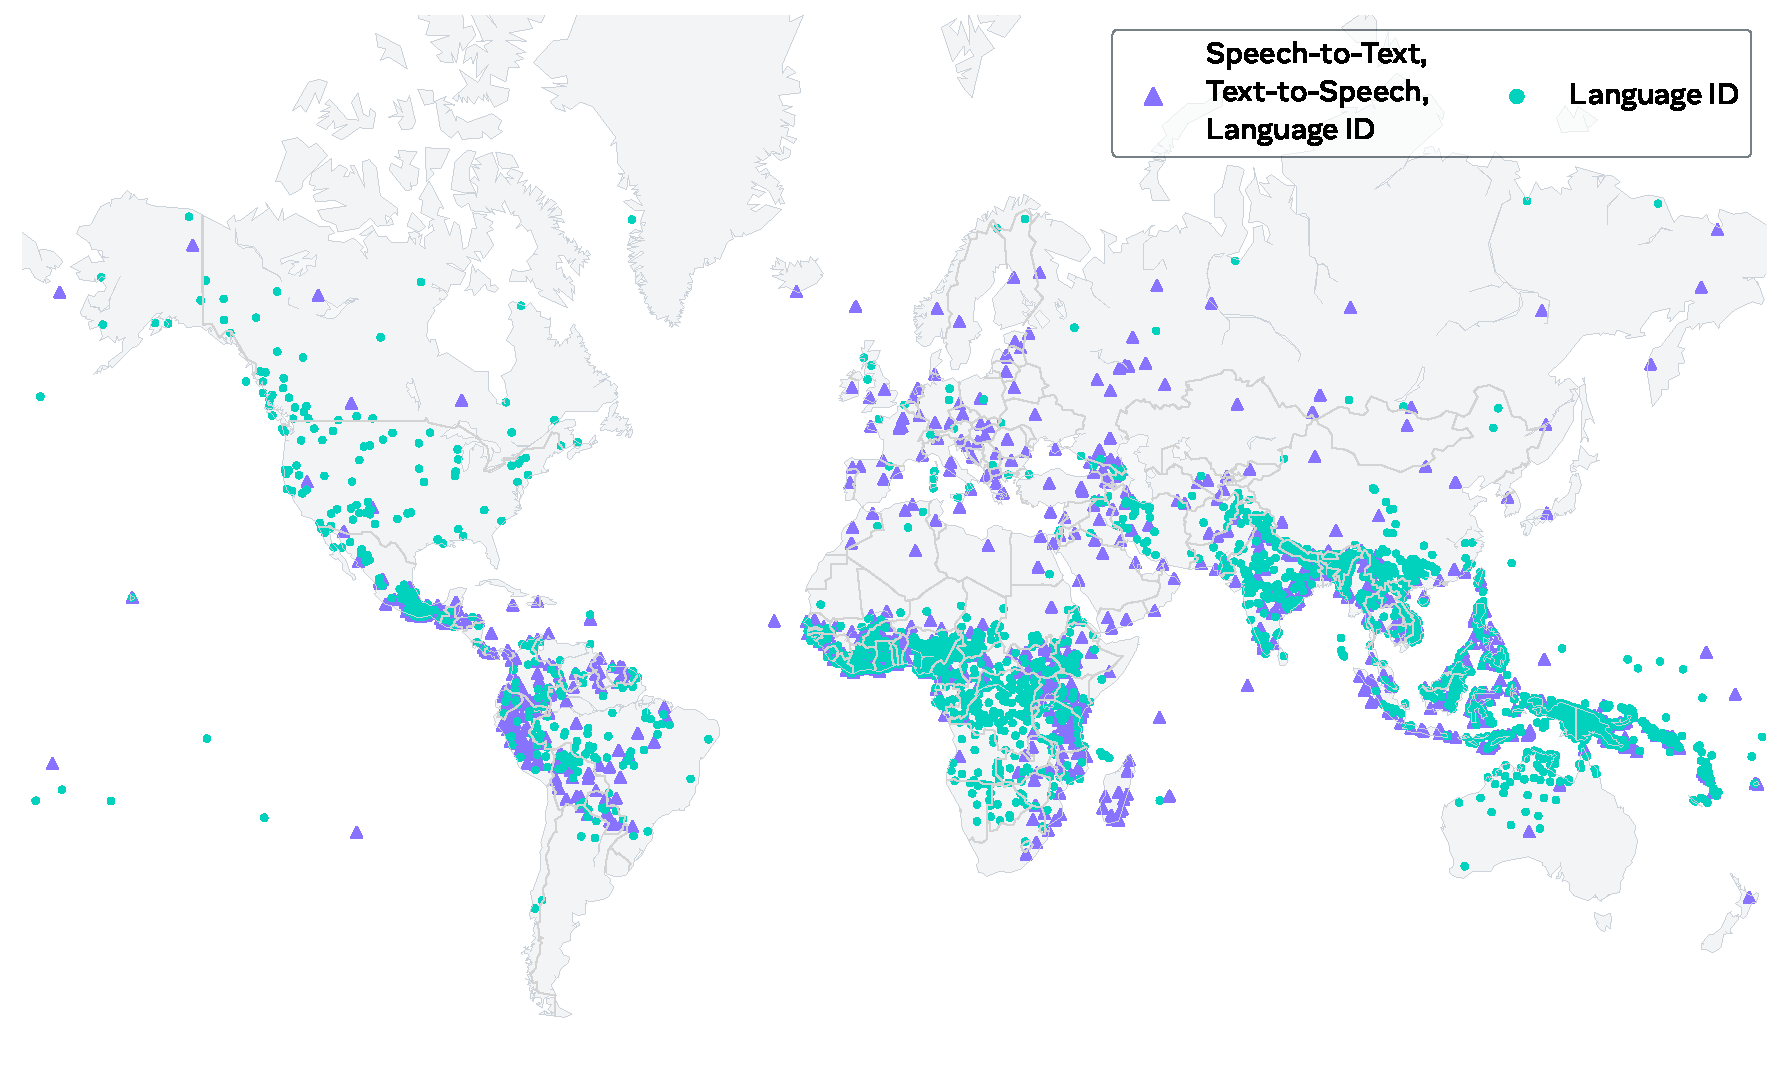
\includegraphics[width=\textwidth]{images/mms_map.pdf} 
\caption{Illustration of where the languages supported by MMS are spoken around the world: 
MMS models support speech-to-text and text-to-speech for \nummmslang{} languages as well as language identification for \numlidlang{} languages.}
\label{fig:map}
\end{figure}
